
\section{Making it whole}
\label{sec:my-patch}

The performance of the current \schedidle{} policy shows us that if we want to
completely isolate LC and BE, we need to put in the final piece to make
\schedidle{} effectively its own scheduling class.

We write a linux patch that does this. The patch intervenes in two places in the
current scheduling process: 1: it ensures that no \schedidle{} entity will be
chosen if there is a runnable \schednormal{} entity (this overrides the fair
share that even a weight 1 process would occasioanlly get in unmodified kernel),
and 2: it tries to steal queued \schednormal{} entities from other cores before
running a \schedidle{} entity.

\begin{figure*}[t]
    \centering
    \begin{subfigure}[t]{0.48\textwidth}
        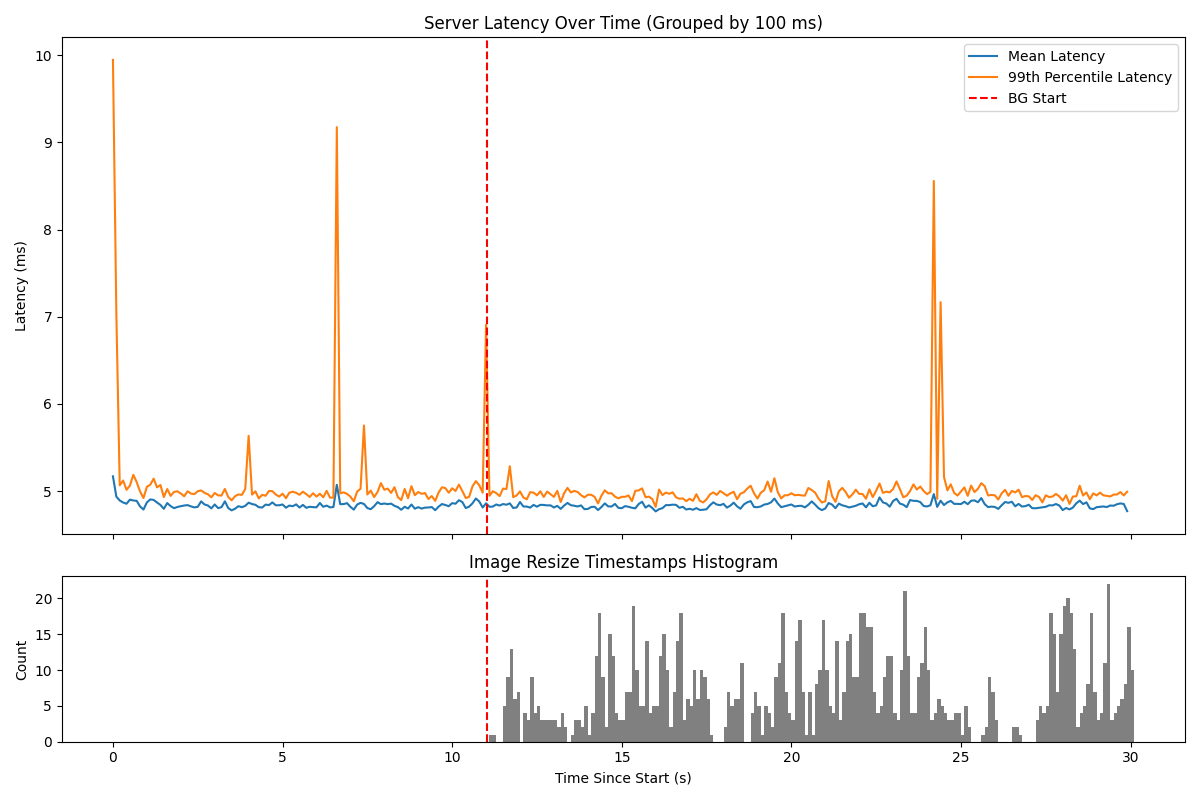
\includegraphics[width=\textwidth]{graphs/patched-idle-low-two.png}
        \caption{Low load}\label{fig:patched-idle-low-two}
    \end{subfigure}
    \hspace{\fill}
    \begin{subfigure}[t]{0.48\textwidth}
        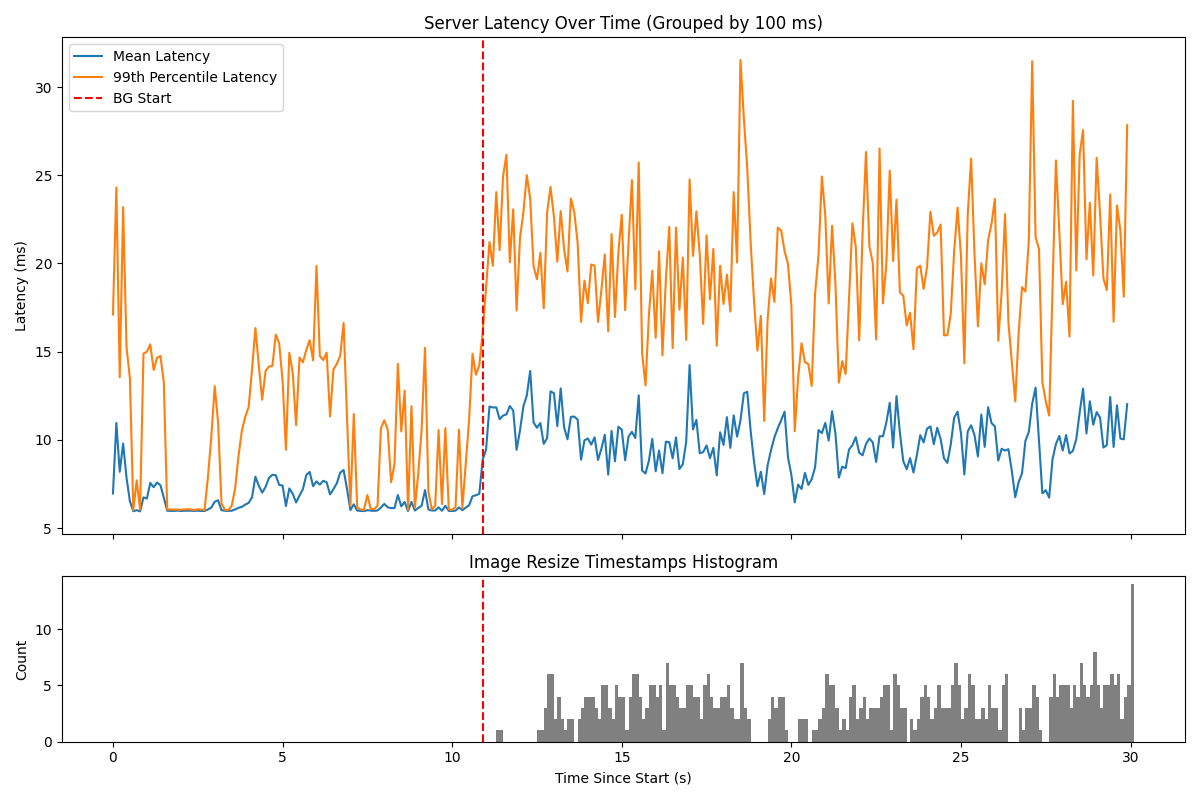
\includegraphics[width=\textwidth]{graphs/unedited-idle-high-two.png}
        \caption{High load}\label{fig:patched-idle-high-two}
    \end{subfigure}
\end{figure*}\label{fig:patched-idle}

We can see the resulting performance in figure~\ref{fig:patched-idle}, and as
desired the latency of the server is completely unaffected by the background
tasks. This does not mean that the background task never runs: the lower graph
still shows iterations of image resizing being done. The difference is that now
the background tasks will reliably get interrupted when the LC server has a
request to process.

